\begin{figure}
        \begin{subfigure}[t]{.5\textwidth}
            \addtocounter{subfigure}{2}
            \centering
            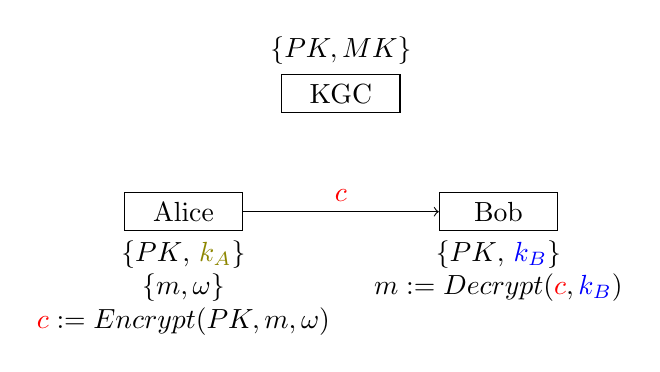
\begin{tikzpicture}[actor/.style={draw, minimum width=1.5cm}]
                \node[actor] (a) at (-2,0) {Alice};
                \node[actor] (b) at (2,0) {Bob};
                \node[actor] (kgc) at (0,1.5) {KGC};
            
                \node[above, align=center] at (kgc.north) {$\{PK, MK\}$};

                \node[below, align=center] at (a.south) {{\{$PK$, $\textcolor{olive}{k_A}$\}}\\$\{m, \omega\}$\\$\textcolor{red}{c}:=\text{Encrypt}(PK, m, \omega)$};
                \node[below, align=center] at (b.south) {\{$PK$, $\textcolor{blue}{k_B}$\}\\$m:=\text{Decrypt}(\textcolor{red}{c},\textcolor{blue}{k_B})$};
                % \node[below, align=center] at (a.south) {$\{PK, k_{A}\}$\\$\{m, \omega\}$};;
                % \node[below, align=center] at (b.south) {$\{PK, k_{B}\}$\\$m:=\text{Decrypt}(c,k_B)$};

                \draw[->] (a) edge node (c) [above] {$\textcolor{red}{c}$} (b);

                % \draw[->] (c.north) -- ++(0,.2) node [anchor=south] {\small $\omega$};
            \end{tikzpicture}
            \caption{Exchange of encrypted messages without involvement of the KGC}
        \end{subfigure}
\end{figure}